\chapter{Moustokouloura}
\label{ch:moustokouloura}
\index{dessert}
\index{cookies}
\index{molasses}
\textit{The Brown Cookies}

Family member: Grandma Eleni

\marginnote[20pt]{\\
    \textbf{Makes 48 cookies} \\
    Prep time: 2-3 hours \\
    Cook time: 12-15 minutes \\
    \vspace*{\baselineskip}

    4 1/2 cups all-purpose flour, sifted \\
    1/2 tsp cinnamon \\
    1/2 tsp cloves \\
    1 tsp baking powder \\
    1 tsp ammonia powder \\
    2 eggs \\
    3/4 cup sugar \\
    1/2 vegetable oil \\
    1/2 orange juice (fresh is better) \\
    1/2 cup molasses \\
}

\newthought{The Brown Cookies} is what we called these cookies. Since \textgreek{μούστο} (grape must) was not easy to find in Canada, Grandma \textgreek{Ελένη} replaced it with molasses. They are a bit tricky to shape, so use some vegetable oil on your hands while shaping.

\begin{enumerate}
    \item In a bowl, mix the cinnamon, cloves, baking powder and ammonia. Add about half of the flour and whisk together. Keep the other flour aside.
    \item In a large mixing bowl, beat the eggs with the sugar. Slowly add the oil, orange juice and molasses while beating.
    \item Add the dry ingredients (half the flour with the spices and baking powder) to the wet ingredients slowly while mixing. Scrape down the sides of the bowl, and let the dough rest for about 15 min.
    \item Restart the mixer and add some of the flour that was kept aside, as much as needed to form a ball. You might not have to use it all.
    \item Place a little bit of vegetable oil in a small bowl and use it to wet hands. Use hands to knead the dough slightly. Dough might be sticky, but use some oil to wet hands. Roll into small balls then into strings, then shape into twists, pretzels and small koulourakia.
    \item Place the shaped cookies onto baking sheets and bake 12-15 minutes on the upper rack at 350\degree F until the tops have a golden color.
\end{enumerate}

\begin{figure}
  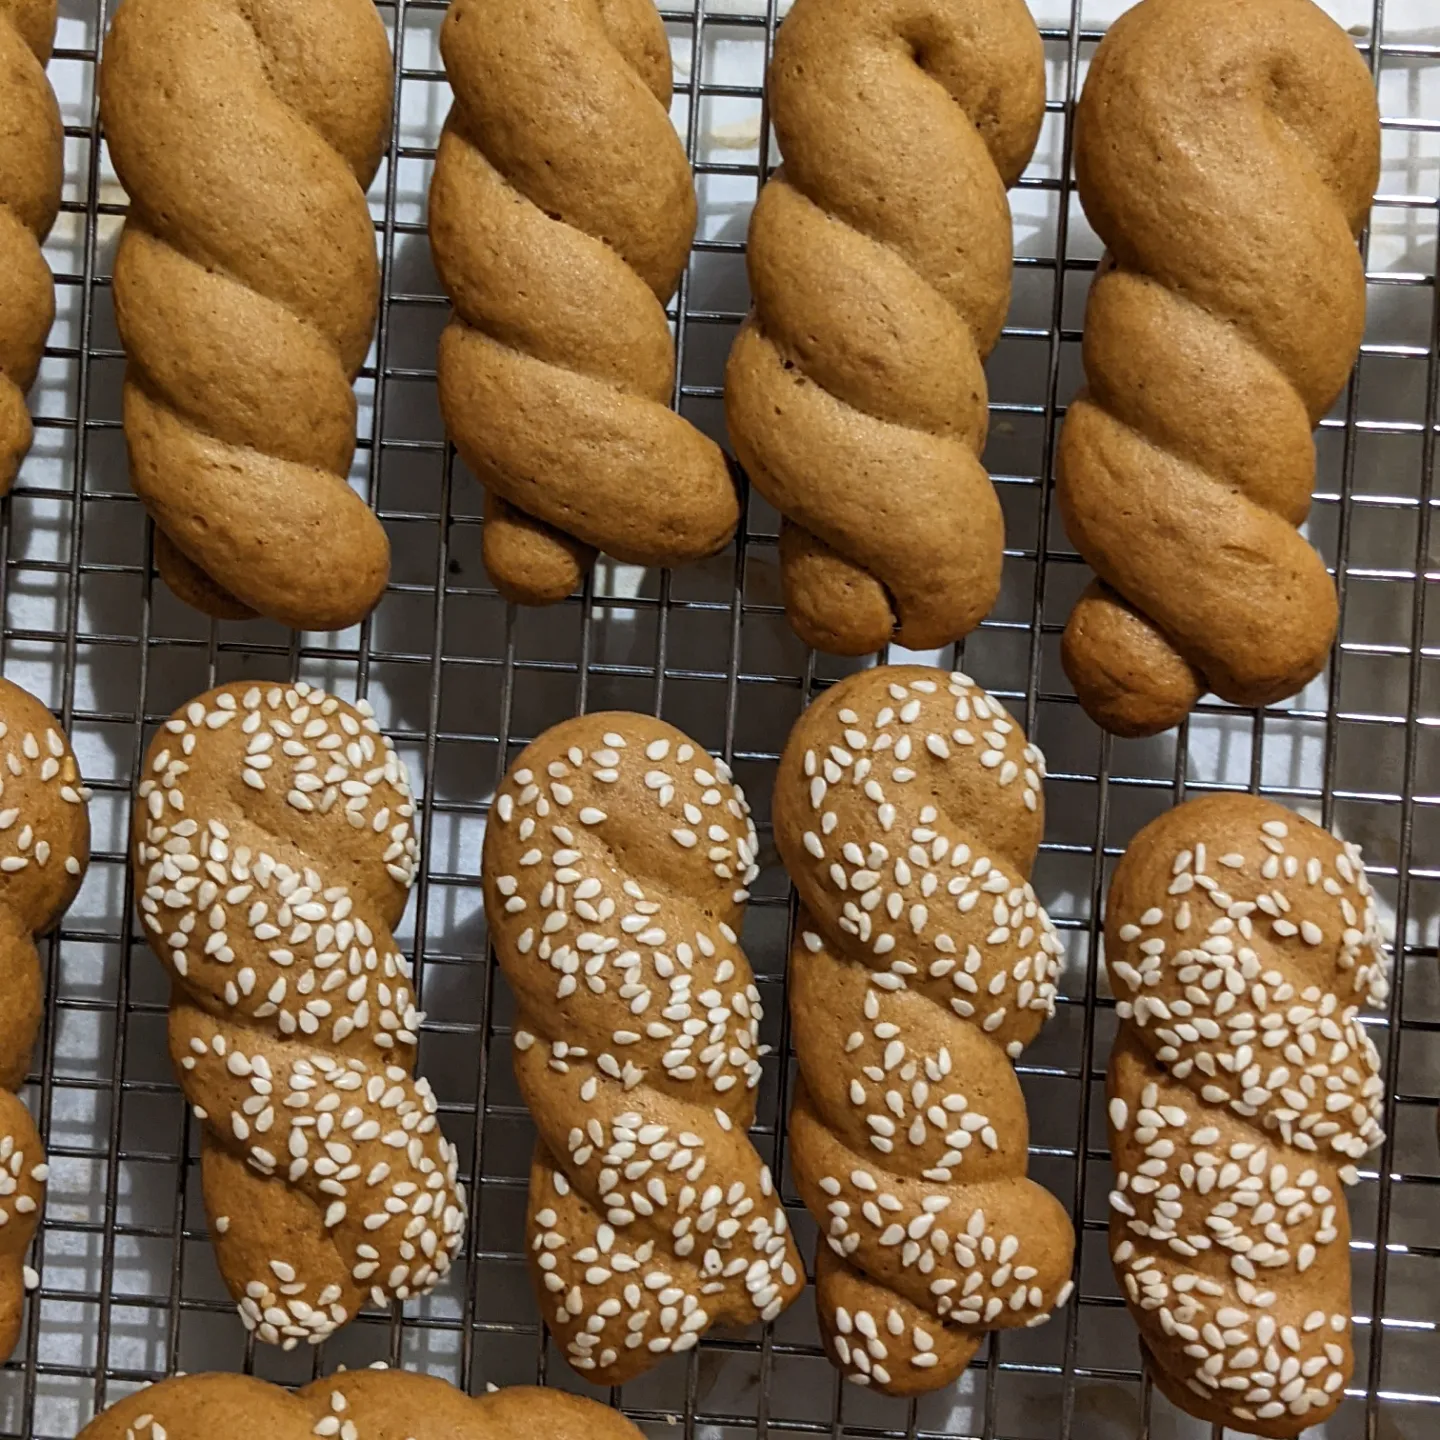
\includegraphics[width=80mm]{monanteras/images/Moustokouloura.jpg}
  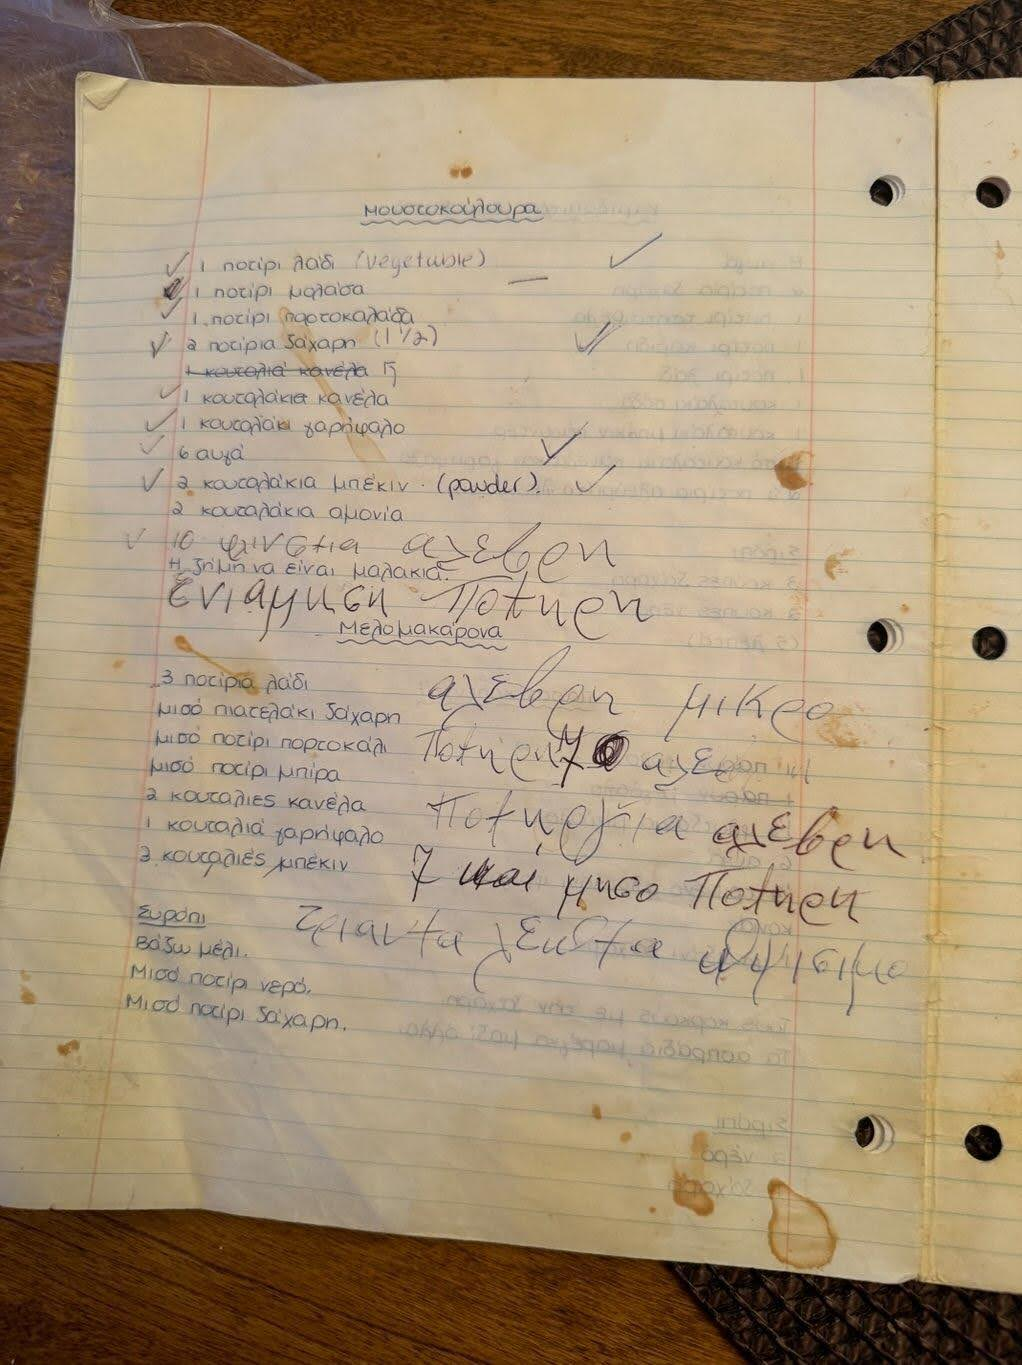
\includegraphics[width=80mm]{monanteras/images/Moustokouloura recipe.jpg}
\end{figure}

\marginnote{
    Eat soon after baking, and once cooled, stored in a large Tupperware. This allows them to be soft and can be kept for a long time if you can resist.
}